\documentclass[12pt]{article}

\usepackage[utf8]{inputenc}
\usepackage[greek, english]{babel}
\usepackage{alphabeta}
\usepackage{libertine}
\usepackage{graphicx}

\title{Algorithms \\ Programming exercise 2}
\author{Κωνσταντίνος Νικολούτσος \\ p3170122}
\date{}



\begin{document}

\maketitle


\section{Ασκηση (Frog-problem)}

\begin{center}
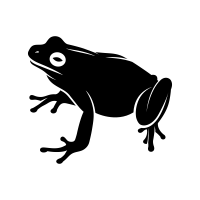
\includegraphics[scale=0.60]{black_frog.png}
\end{center}


\subsection{Αναδρομική εξίσωση}
Η αναδρομική εξίσωση προκύπτει εύκολα εφόσον εχουμε κάνει τον αλγόριθμο με bottom-up approach (Θα το γράψουμε με μαθηματική μορφη). \\\\
$F_i = 1 + j, $ τέτοιο ώστε,  $j = \min_{j < i} (F_j)*bool $ \\\\
Οπου, το bool ειναι είτε 1 είτε 0 και εξαρτάται απο το αν στο νούφαρο που εξετάζουμε ο βάτραχος μπορει να πάει στο νουφαρο που βρισκόμαστε.(Ειναι 1 οταν γινεται να παει)(Δηλαδη στην αναδρομή το επόμενο βγαινει φιλτραροντας τα προηγουμε αναλογα με το αν μπορει ο βατραχος να πηδηξει σε αυτα και μετα παιρνουμε το ελαχιστο απο αυτα και προσθετουμε 1) 


\subsection{Πολυπλοκότητα χρόνου}
Ειναι προφανές οτι η πολυπλοκότητα χρόνου ειναι $Ο(n^2)$
Αφου για καθε leaf που βρισκεται στην θεση position κανουμε (αθροισμα απο ενα εως position βηματα).
Η απόδειξη ειναι εύκολη αφου τα βήματα που κανει ο αλγόριθμος μας αμα τα μετρήσουμε ειναι:\\
$$\sum_{n=0}^{N} n := O(n^2)$$\\
Που αυτο γνωριζουμε οτι ειναι πολυπλοκότητας $O(n^2)$\\

\subsection{Μια μικρή αναβάθμιση στον αλγόριθμο}
Θα μπορούσαμε για καθε φύλλο αντι να ξεκινάγαμε την διαδικασία απο την αρχή, να πηγαιναμε απλα πισω οσες θεσεις ειναι η μεγιστη τροφη στο προβλημα μας. Nevertheless, αυτο θα μας εδινε καλυτερο χρονο αλλα θα ειχαμε ιδια πολυπλοκοτητα μεγαλου ομικρον(για μεγαλη εισοδο)



\section{Ασκηση (Dietologist-problem)}
\begin{center}
	
\includegraphics[scale=0.45]{diet.png}
\end{center}


\subsection{Αναδρομική εξίσωση}


\[ 
F{i,j}= \left\{
\begin{array}{ll}
0 & i=0,j=0 \\
max(F{i-1,j}, cal(i-1) + F{i-1, j - weight(i-1)})& can\_be\_included\\
F{i-1,j}& cannot\_be\_included \\
\end{array} 
\right. 
\]

Η παραπάνω αναδρομική εξίσωση ειναι απλοποιημένη(Αν θελετε περισσοτερη λεπτομερεια δειτε τον κωδικα). Με λόγια αυτο σημαίνει οτι φτίαχνουμε εναν πινακα [C+1][T+1] και τον γεμίζουμε κάνωντας κατα γραμμή κάνωντας τα εξείς. Ας γεμίσουμε την γραμμή i για να το καταλαβουμε. Αν το αντικειμενο i δεν χωραει να μπει(οι θερμιδες δεν επαρκουν) τοτε παιρνουμε την πανω τιμη που βρισκοταν στον δισδιαστατο πινακα. Αν ομως χωραει τοτε παιρνουμε το max μεταξυ του απο πανω και του να συμπεριλαμβαναμε το αντικειμενο μαζι με οτι αλο μπορουσαμε( πανω μειωμενο κατα θερμιδες αυτου που βαλαμε). Αυτα τα προβλήματα δεν ειναι και τοσο ευκολο να τα εξηγείς γραφοντας ενα κειμενο, συνήθως χρειάζονται ενα animation!



\subsection{Πολυπλοκότητα χρόνου} 
Η πολυπλοκότητα χρόνου ειναι της ταξης $Ο(C*N)$ οπου C,Ν το πληθος των θερμιδων για το οποιο ζητειτε να βρουμε μενου
και το πληθος των αντικειμενων που εχουμε στην διαθεση μας αντιστοιχα!

\newpage
\section{Ασκηση greedy 1}

\subsection{Λύση}

\begin{itemize}
	\item Ταξινομησε τα διαστηματα αναλογα με το finish point σε αυξουσα σειρα(mergeSort ή HeapSort)
	\item Παρε το διαστημα που τελειωνει πρωτο
	\item Βαλε ενα σημειο εκει που τελειώνει.
	\item Βγαλε απο το παιχνίδι τα διαστηματα που εχουν καλυφθει.(Αποθηκευσε τα σε ουρα)
	\item goto bullet 2 μεχρι οτου δεν υπαρχει ακαλυπτα intervals
	
	(*Αν για καποιο σημειο δεν υπαρχει διάστημα το οποιο το περιέχει τοτε ο αλγόριθμος μας θα επιστρέψει οτι δεν γίνεται να καλυφθουν ολα τα σημεία και θα γυρίσει την τρέχων λυση. Οπως μου απαντήσατε στο forum του eclass)
	
\end{itemize}


\subsection{Πολυπλοκότητα χρόνου} 
Η πολυπλοκότητα χρόνου ειναι της ταξης $Ο(n*log(n))$ (χρησημοποιώντας mergesort) .
Τα βηματα για να λυθει αφου εχει γινει ταξινομιση ειναι n. Αρα το πιο αργο σημειο του αλγορθμου εινια η ταξινομιση

\subsection{Απόδειξη ορθότητας} 
Θα χρησιμοποιησουμε το επιχειρημα της ανταλλαγης. \\
Εστω οτι υπήρχε μια αλλη Optimum λυση και μεχρι καποιο σημειο ειχαμε επιλέξει τα ιδια σημεία. Εστω τωρα οτι σε ενα σημειο ειχαμε επιλεξει διαφορετικα, τοτε αν αντικαθιστουσε η βελτιστη λυση το σημειο το δικο μου θα εβγαζε καλυτερη λυση (αφου θα καλυπτει περισσοτερα σημειο) , το οποιο ειναι ατοπο αρα η λυση μου εινια ιδια με το Optimum.

\newpage
\section{Ασκηση greedy bonus}

\subsection{Λύση}
Πριν ξεκινήσουμε να πουμε την λύση ας ορίσουμε μια μέθοδο Interval findBestInterval(Point p, Interval[] intervals) η οποια μας δινει για ενα συγκεκριμενο σημείο το interval που πρεπει να παρουμε ωστε να βγαλουμε σιγουρα optimum λυση.\\
Πως γινεται η επιλογή;; Η μεθοδο επιλέγη το interval το οποιο καλυπτει πρωτα το σημειο και επισης καλυπτει οσο το δυνατο δεξια απο το σημειο.\\
Οποτε αφου ξεκαθαρισαμε με αυτο ας πουμε τα βηματα που πρεπει να ακολουθησουμε ωστε να λυθει το προβλημα:

\begin{itemize}
	\item Κανε ταξινόμιση στα σημεία σε αυξουσα σειρα (mergeSort ή HeapSort)
	\item Επιλεξε το πρωτο σημειο(το οποιο δεν εχει καλυφθει) και κανε την μεθοδο findBestInterval
	\item Διεγραψε το interval που χρησιμοποιηθηκε καθως και τα σημεια τα οποια καλυπτει
	\item Επαναλαβε, επαλαβε μεχρι οτου δεν υπαρχουν αλλα σημεια

\end{itemize}




\subsection{Πολυπλοκότητα χρόνου} 
Η πολυπλοκότητα του συγκευκριμένου αλγορίθμου ειναι ανηκει στην πολυωνυμικη κλάση. Πιο συγκεκριμένα, η πολυπλοκότητα ειναι ιση με $O(n*Μ)$) οπου n και M ο αριθμος των σημειων και των διαστημάτων αντίστοιχα. Αυτο συμβαινει διότι για να λυθει αυτο θα πρεπει να υλοποιήσουμε 2 for loops τα οποια θα βρισκεται το ενα μεσα στο αλλο.




\subsection{Απόδειξη ορθότητας} 
Εστω οτι ειχαμε την βελτιστη λυση τοτε αν διαφοροποιουταν σε ενα σημειο απο το δικο μας θα μπορουσαμε να την ανταλλασαμε και η βελτιστη να ηταν ακομα βελτιστη.
Αρα αυτο σημαινει οτι εχουμε την βελτιστη λυση. Επισης εινια πολυ λογικο να εχουμε την βελτιστη λυση αφου ειμαστε biased προς τα διαστηματα που εχουν την ταση να πηγαινουν περισσοτερο δεξια στον χωρο(δηλαδη καλυπτουν οσο πιο καλα γινεται τον χωρο)


\end{document} 
